\documentclass[12pt]{article}
% Эта строка — комментарий, она не будет показана в выходном файле
\usepackage{ucs}
\usepackage[utf8x]{inputenc} % Включаем поддержку UTF8
\usepackage[russian]{babel}  % Включаем пакет для поддержки русского языка
\usepackage{amsmath}
\usepackage{amssymb}
\usepackage{mathtools}
\usepackage{graphicx}
\graphicspath{ {/Users/sergmiller/Documents/tex/formal/automatlang/} }

\title{Домашнее задание № 3}
\date{\today}
\author{Сергей Миллер 494}

\begin{document}
 	\maketitle
	\textbf{Задача 1.}
 	
  	\textbf{a)}
      Построим недетерминированный автомат(вершина серого цвета - начальная, вершины в виде двойного круга - конечные).
      Очевидно, что каждый блок из $a$ четной длины имеет нечетное вхождение подслова  $aa$. Тогда построим автомат в котором старт и финиш находятся на цикле, в котором любой путь до финиша проходит через нечетное количество групп с четным числом букв $a$. Очевидно, что в остальных местах слова может быть любая последовательность из $b$, между которыми любое число групп из $a$ нечетной длины.

      %\includegraphics[width=0.5\linewidth]
      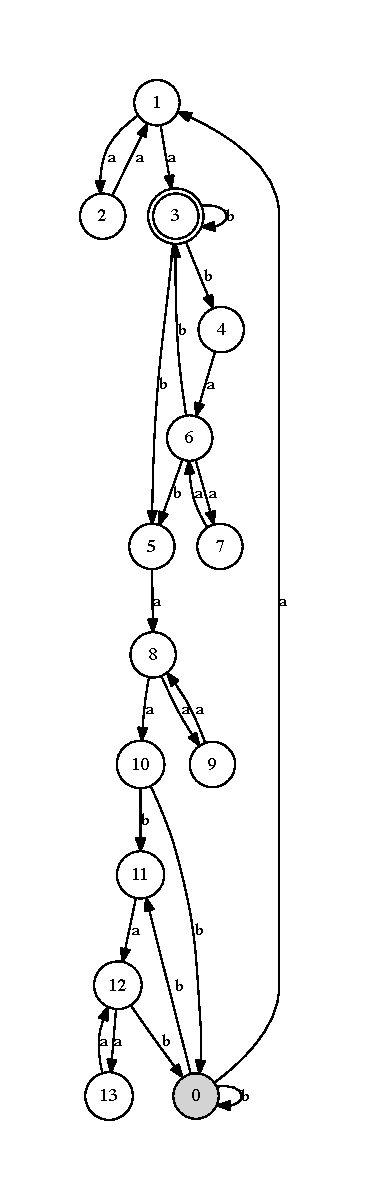
\includegraphics{nfae5.pdf}

      \text{Построим ДКА:}

    \begin{array}{c|c|c}
      0 & a & 1 \\
      0 & b & 0,11 \\
      \hline
      1 & a & 2,3 \\
      \hline
      0,11 & a & 1,12 \\
      0,11 & b & 0 \\
      \hline
      2,3 & a & 1 \\
      2,3 & b & 3,4,5 \\
      \hline
      1,12 & a & 2,3,13 \\
      1,12 & b & 0 \\
      \hline
      3,4,5 & a & 6,8 \\
      3,4,5 & b & 3,4,5 \\
      \hline
      2,3,13 & a & 1,12 \\
      2,3,13 & b & 3,4,5 \\
      \hline
      6,8 & a & 7,9,10 \\
      6,8 & b & 3,5 \\
      \hline
      7,9,10 & a & 6,8 \\
      7,9,10 & b & 0,11 \\
      \hline
      3,5 & a & 8 \\
      3,5 & b & 3,4,5 \\
      \hline
      8 & a & 9,10 \\
      \hline
      9,10 & a & 8 \\
      9,10 & a & 0,11 \\

    \end{array}

    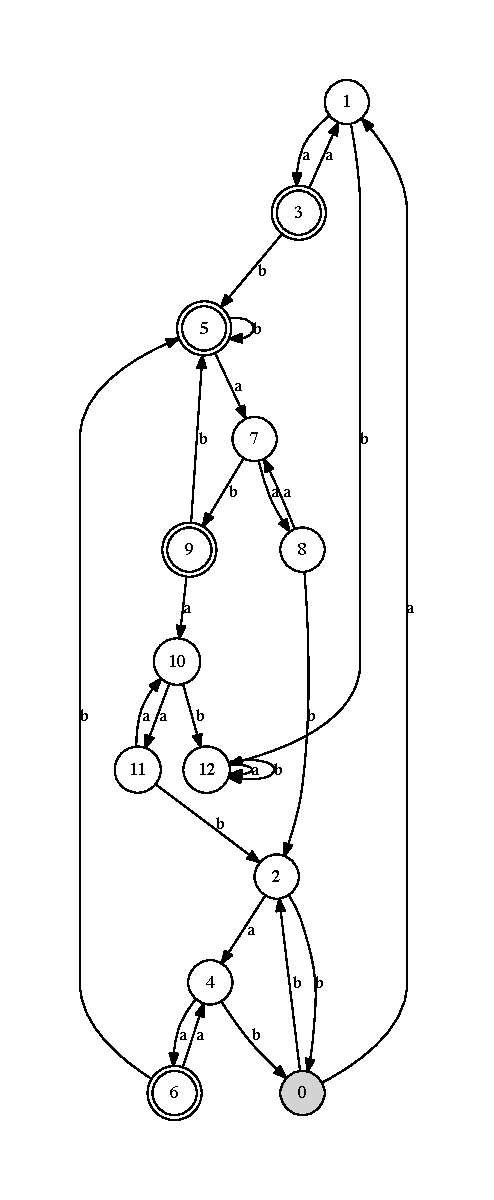
\includegraphics{dfa3.pdf}

       \begin{array}{c|c|c|c|c|c|c|c|c|c|c|c|c|c}
      - & 0 & 1 & 2 & 3 & 4 & 5 & 6 & 7 & 8 & 9 & 10 & 11 & 12 \\
      \hline
      a & 1 & 3 & 4 & 1 & 6 & 7 & 4 & 8 & 7 & 10 & 11 & 10 & 12 \\
      b & 2 & 12 & 0 & 5 & 0 & 5 & 5 & 9 & 2 & 5 & 12 & 2 & 12 \\
      \hline
      a & A & B & A & A & B & A & A & A & A & A & A & A & A \\
      b & A & A & A & B & A & B & B & B & A & B & A & A & A \\
      \hline
      a & C & D & C & C & D & B & C & A & B & A & A & A & A \\
      b & A & A & A & D & A & D & D & D & A & D & A & A & A \\
      \hline
      a & B & C & B & B & C & E & B & F & E & G & G & G & G \\
      b & A & G & A & D & A & D & D & H & A & D & G & A & G \\
      \hline
      a & $B_1$ & C & $B_2$ & $B_1$ & C & E & $B_2$ & F & E & $G_1$ & $G_2$ & $G_1$ & $G_1$ \\
      b & A & $G_1$ & A & D & A & D & D & H & A & D & $G_1$ & A & $G_1$ \\ 
  

    \end{array}

    Видно, что все вершины разбиваются на отдельные классы, а значит полученный ДКА является минимальным.
   
\end{document}